\documentclass[conference,9pt,letterpaper]{IEEEtran}
\usepackage[T1]{fontenc}
\usepackage{newtxtext,newtxmath}
\usepackage{graphicx}
\usepackage{booktabs}
\usepackage{amsmath}
\usepackage{array}
\usepackage{xcolor}
\usepackage{soul}
\DeclareRobustCommand{\pending}[1]{{\sethlcolor{yellow}\hl{#1}}}
\setlength{\abovecaptionskip}{3pt}
\setlength{\belowcaptionskip}{2pt}
\setlength{\intextsep}{6pt plus 1pt minus 1pt}
\setlength{\textfloatsep}{7pt plus 1pt minus 1pt}
\setlength{\floatsep}{6pt plus 1pt minus 1pt}
\usepackage{cite}
\usepackage{url}
\usepackage{stfloats}
\usepackage{balance}
\usepackage{capt-of}
\usepackage{float}
\usepackage{needspace}
\setcounter{dbltopnumber}{3}
\renewcommand{\dbltopfraction}{0.85}
\renewcommand{\textfraction}{0.10}
\newcommand{\mecc}{\textsc{MECC}}
\newcommand{\BH}{B_{\mathrm H}}
\newcommand{\BC}{B_{\mathrm C}}
\newcommand{\KH}{K_{\mathrm H}}
\newcommand{\KC}{K_{\mathrm C}}
\newtheorem{proposition}{Proposition}
\title{MECC: Single-GPU MoE Inference with\protect\\Compiler-Guided Three-Tier Expert Caching}
% Anonymous review copy: no author names or affiliation spacer rows.
\author{}
\usepackage[hidelinks]{hyperref}
\hypersetup{pdftitle={MECC: Single-GPU MoE Inference with Compiler-Guided Three-Tier Expert Caching},pdfauthor={}}
\begin{document}
\maketitle\raggedbottom
\begin{abstract}
Single-GPU MoE inference reads expert weights from HDD when a task's HBM and host allocation cannot retain the model. Initial placement and later GPU evictions determine how often these reads recur. We present MECC, the MoE Expert Cache Compiler, to connect layer-wise initial allocation with joint HBM/CPU retention. The compiler emits capacities and ranked expert IDs. The runtime promotes selected experts and retains GPU victims on the host. Delivery orders reads and copies before consumption. In single-run FP16 Mixtral-8x7B measurements on one A100, MECC with uniform initialization takes 7.38~s per decode token. Decode speedups are 1.77$\times$ over streaming and 2.95$\times$ over fixed CPU retention. Sample perplexity matches these controls.
\end{abstract}

\begin{IEEEkeywords}
Mixture of experts, single-GPU inference, expert offloading, three-tier caching, hardware/software co-design.
\end{IEEEkeywords}

\section{Introduction}
Mixture-of-experts (MoE) models expand parameter capacity while selecting a subset of experts for each token~\cite{shazeer,switch,mixtral,deepseekmoe}. Sparse execution reduces arithmetic. Every expert can still be selected by a later token. A single GPU may lack the HBM needed to retain that pool. A serving task may also receive less host memory than the server contains. This setting arises when jobs share a host or reserve resources for separate model instances. Expert demand can then reach HDD after missing both fast tiers. Every such miss adds weight delivery to the layer's execution path. The fast tiers avoid different parts of that path. An HBM hit avoids both the cold read and H2D. A host hit avoids the cold read but still needs H2D. A placement decision therefore changes where a later request begins its delivery. A token crosses many MoE layers, so these delays can recur throughout decoding. Retaining weights across tokens can avoid repeated reads without changing the router or precision. We study how to allocate that retention capacity and update its contents during inference. The resource constraint belongs to the serving task: physical server capacity alone does not determine which weights the task can retain.

Expert parallelism distributes the expert pool over several GPUs~\cite{deepspeedmoe,tutel,flashmoedist}. Offloading systems instead manage transfers, host execution, and expert residency~\cite{offloading,moeinfinity,fiddler,lightning,promoe}. MoE-CORE combines layer-wise allocation, profile initialization, and online replacement~\cite{core}. SSD-LLaMA combines bounded RAM/VRAM caches with storage delivery~\cite{ssdllama}. Edge FlashMoE studies replacement under device-memory constraints~\cite{flashmoe}. These systems establish the importance of deciding which experts remain accessible after execution. MECC examines a specific coupling: an offline layer allocation supplies the initial state of a joint HBM/CPU retention rule. Initial coverage determines the first demand reads. The plan and the eviction rule affect different request segments. Loading a frequently selected expert can reduce early reads. Its first GPU eviction creates a later choice: retain it on the host or fetch it again. The host admission can also displace another expert. A plan's initial hit rate does not describe this sequence of choices. Promotion and victim retention determine whether later selections require another cold read. Figure~\ref{fig:intro} isolates the latter decision in local A100 controls. Independent caches take 32.94~s per decode token, versus 7.38~s for joint retention at the same nominal slots and initialization. Their all-phase HDD-demand shares are 47.9\% and 12.5\%. The shared loader and initial state connect this difference to the local retention rules.

\begin{figure}[H]
\centering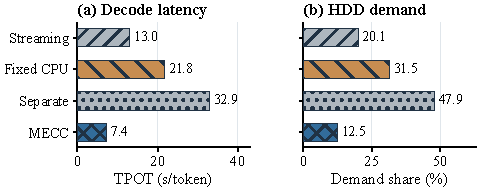
\includegraphics[width=\columnwidth]{measured_figures/intro_evidence.pdf}
\par\nointerlineskip
\caption{Local single-A100 cache controls on Mixtral-8x7B. Separate denotes independent HBM/CPU management. All policies use the same nominal slots, initialization, and eight-prompt input. HDD demand spans all instrumented phases; each policy has one run.}
\label{fig:intro}
\end{figure}

We present \mecc{}, the MoE Expert Cache Compiler, for this allocation and retention problem. The compiler takes model metadata, task allowances, and layer profiles. It compares the next uncovered rank in each layer and emits HBM/CPU capacities with ordered expert IDs. Initialization loads those IDs into the fast tiers. During inference, the original router supplies demand. An HBM hit changes recency. A CPU hit promotes its expert and preserves the displaced HBM expert on the host. A cold admission follows the same promotion/demotion rule and can remove a host victim. Capacities remain fixed while resident identities follow the stream. The plan retains layer IDs, so equal expert indices in different layers remain separate objects. An expert can enter HBM even when calibration never selected it. Delivery resolves the selected experts' read and copy dependencies before their GPU consumers execute. The implementation batches cold reads during prefill and uses demand delivery during decode. This separates three responsibilities: selecting an initial state, retaining experts after tier crossings, and making selected weights available for computation. The compiler's output becomes the runtime's starting state; observed requests determine its later membership.

This paper makes three contributions.
\begin{list}{}{\setlength{\leftmargin}{16pt}\setlength{\labelwidth}{14pt}\setlength{\labelsep}{2pt}\setlength{\itemsep}{3pt}\setlength{\topsep}{3pt}}
\item[(1)] \textbf{Compiling initial residency:} we specify a layer-wise plan with capacities and expert IDs. A marginal-coverage scan allocates slots under fixed expert allowances.
\item[(2)] \textbf{Preserving cross-tier reuse:} we connect that plan to a joint promotion/demotion rule. We separate logical membership from the host mirrors and temporary copies used by delivery.
\item[(3)] \textbf{Characterizing the decisions:} we compare placement, retention, transfer exposure, and workload sensitivity under a shared inference interface. On one A100, uniform-initialized MECC takes 7.38~s/token, versus 13.04 for streaming and 21.75 for fixed CPU retention. These are local policy controls. The evaluation separates initial coverage from later replacement and examines the latency paid for using one accelerator.
\end{list}
\twocolumn[{
\begin{minipage}{\textwidth}
\centering
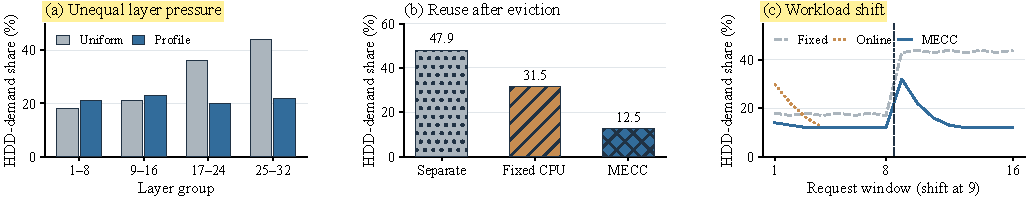
\includegraphics[width=\textwidth]{completion_figures/motivation_evidence.pdf}\par
\vspace{2pt}
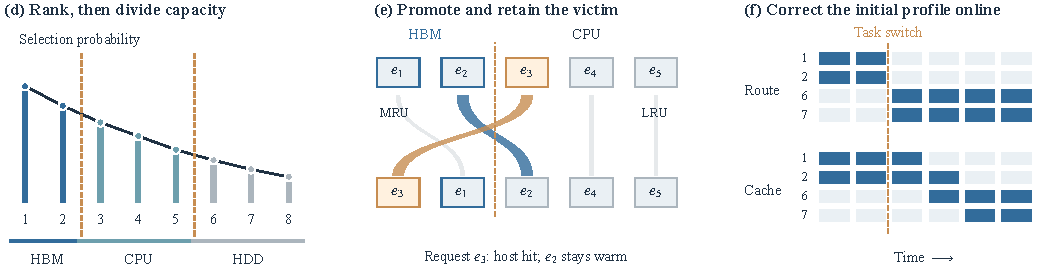
\includegraphics[width=\textwidth]{measured_figures/insights_lower.pdf}
\par\nointerlineskip
\captionof{figure}{Motivation evidence and matching insights. (a--c) compare layer pressure, cross-tier reuse, and workload change; (b) counts A100 demand across all phases. (d--f) show layer-specific capacity cuts, joint victim retention, and online membership updates.}
\label{fig:insights}
\vspace{5pt}
\end{minipage}
}]
\section{Background}
\label{sec:background}
\subsection{Sparse Execution, Full Weight Capacity}
An MoE layer contains a router and a bank of experts. The router selects a small subset for each token, and their weighted outputs form the layer result~\cite{shazeer,switch,gshard}. Mixtral and the DeepSeek family use this separation between active arithmetic and total model capacity~\cite{mixtral,deepseekmoe,deepseekv2,deepseekv3,mixtral22}. Expert identity includes the layer: equal indices in different layers refer to different weights. A generated token passes through successive layers, so expert demand is revealed incrementally during the forward pass. Autoregressive decoding revisits these layers with potentially different selections. Residency changes the location of an immutable expert, while its router score and function remain unchanged.

\subsection{Expert Residency on One GPU}
With enough aggregate HBM, expert parallelism places experts on different GPUs and moves token activations to their owners~\cite{deepspeedmoe,tutel,megablocks,flashmoedist,harmoeny}. A single-GPU deployment instead moves selected weights through the memory hierarchy. Dense layers, activations, and the KV cache compete with experts for HBM; KV management is complementary to expert caching~\cite{pagedattention,sglang}. A CPU hit needs a host-to-device (H2D) copy. An HDD miss first reads the expert into host memory. Heterogeneous inference systems expose these capacity and delivery choices~\cite{flexgen,dsinference,zeroinfinity,llmflash,powerinfer}. We use immutable FP16 experts and retain backing weights on HDD. A resident copy avoids a later cold read, making the history of expert reuse relevant even though routing remains sparse. Below full fast-tier coverage, requests can miss both HBM and CPU. MECC addresses this regime by preserving useful copies that avoid another HDD read.

\section{Motivation and Insights}
\label{sec:challenges}
\subsection{Allocating Slots by Marginal Demand}
A slot can cover different request mass in different layers. Uniform allocation gives each layer the same capacity, even after its hottest experts fit. Figure~\ref{fig:insights}(a,d) connects the resulting pressure to a per-layer capacity cut. The next uncovered expert determines the gain from another slot. Comparing that gain across layers allocates capacity where it covers more demand. Ranking within each layer then determines the initial IDs. Capacity and identity are separate outputs: one sets the room available to a layer, and the other fills it. Routing locality across models has also been studied independently~\cite{routingconsistency}.

\subsection{Preserving Reuse after GPU Eviction}
A GPU eviction changes an expert's location before it determines the expert's next use. If the host retains the weights, another selection avoids HDD. Figure~\ref{fig:insights}(b,e) shows the promotion/demotion decision. Promotion vacates one CPU position as the HBM victim loses its GPU position. Joint retention reuses that host position for the victim. The local independent-cache control reports 47.9\% HDD demand, versus 12.5\% for joint retention across all instrumented phases. This comparison concerns the specified policies under the same initial slots. It motivates preserving the victim's place in the combined reuse order, rather than discarding its history at the HBM boundary.

\subsection{Updating Residency beyond Calibration}
A profile summarizes calibration inputs. The next prompt can select a different expert set before a fixed initial placement changes. Figure~\ref{fig:insights}(c,f) pairs the demand shift with an update of resident IDs. The compiler supplies capacities and a starting membership. Recency then changes membership within those capacities. Initial coverage controls early reads; online admission controls the response to later selections. These are separate time intervals in one cache lifecycle. A task switch can expose the distinction even when both methods start with the same profile. Updating IDs from actual requests lets the runtime respond without compiling a new plan or predicting a later gate.

\twocolumn[{
\begin{minipage}{\textwidth}
\section{Overview}
\label{sec:overview}
\centering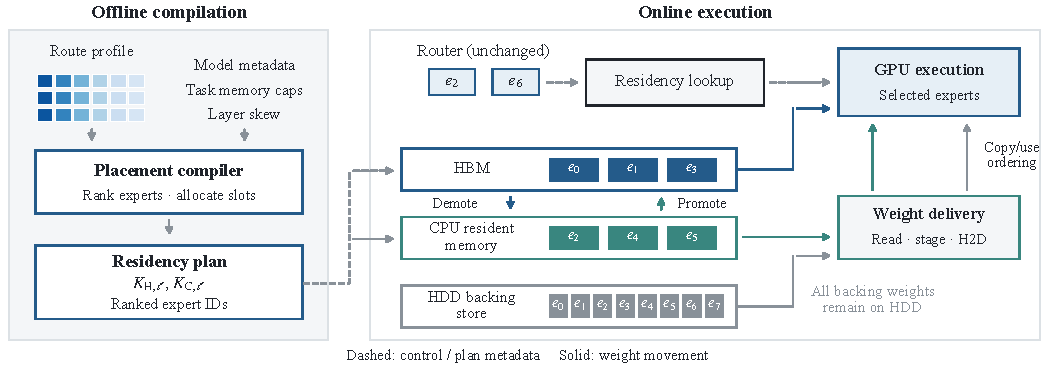
\includegraphics[width=\textwidth]{figures/fig01_overview.pdf}
\par\nointerlineskip
\captionof{figure}{MECC framework. The placement compiler emits per-layer capacities and ranked IDs. Online execution resolves unchanged router selections against HBM, CPU resident memory, and HDD, then delivers weights before their GPU consumers. Dashed arrows carry control or plan metadata; solid arrows move weights.}
\label{fig:overview}

\vspace{8pt}
\end{minipage}
}]

Figure~\ref{fig:overview} follows one model from preparation to inference. Offline profiling supplies layer/expert counts and skew parameters. The compiler combines those inputs with model metadata and task allowances. Its plan records per-layer capacities, ordered IDs, and initial tiers. Initialization reads the specified experts from HDD and populates HBM and CPU. The backing store retains the complete pool.

At each MoE layer, the gate produces selected IDs and weights. Residency lookup chooses HBM, CPU, or HDD as the source. Promotion makes the requested expert available on the GPU. Demotion preserves an HBM victim on the host when the retention rule admits it. Read and copy dependencies then order execution before output aggregation. Each generated token repeats this layer sequence; later tokens reuse the resulting resident state.

The interfaces separate what stays fixed from what changes. The plan fixes per-layer capacities. Accesses change membership and recency. Delivery controls when weights can be consumed. Placement comparisons therefore hold the runtime rule fixed. Retention comparisons hold initial capacities and IDs fixed. Scheduling comparisons use the same demand and resident state. This decomposition links the framework to the comparisons in Section~\ref{sec:evaluation} without treating any one component as a substitute for the others.

\section{Method}
\label{sec:method}
\subsection{Compiling Capacities and Initial Identities}
\begin{figure}[H]
\centering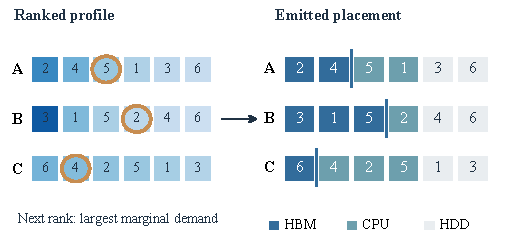
\includegraphics[width=\columnwidth]{method_redesign/compile_frontiers.pdf}
\par\nointerlineskip
\caption{Compiling the initial state. The left grid contains ranked per-layer demand; circles mark the next uncovered candidates. Shared HBM/CPU slot allowances produce different cuts in the emitted rows. A, B, and C identify different layers. Values and slot counts are schematic.}
\label{fig:compile}
\end{figure}

Consider $L$ MoE layers with $N_\ell$ experts per layer. The evaluated models use equal-size experts and equal top-$k$ across layers. Let $s$ be expert size and let $B_{\mathrm H},B_{\mathrm C}$ be logical expert allowances. They supply $S_{\mathrm H}=\lfloor B_{\mathrm H}/s\rfloor$ HBM slots and $S_{\mathrm C}=\lfloor B_{\mathrm C}/s\rfloor$ CPU slots. Dense weights, activations, mirrors, and staging are separate allocations.

The compiler takes an expert order and a skew parameter $\alpha_\ell$ for each layer. Profile counts determine expert order; a discrete Zipf model supplies the marginal slot score:
\begin{equation}
q_{\ell,r}=\frac{r^{-\alpha_\ell}}{\sum_{j=1}^{N_\ell}j^{-\alpha_\ell}},
\qquad p_{\ell,r}=q_{\ell,r}/L.
\end{equation}
Here $r$ is a rank within one layer, not an expert ID shared across layers. Equal top-$k$ gives equal layer selection mass. Sorting counts preserves the mapping from each rank to its original expert ID.

Figure~\ref{fig:compile} shows the resulting cuts. A valid plan obeys $\sum_\ell K_{\mathrm H,\ell}\le S_{\mathrm H}$, $\sum_\ell K_{\mathrm C,\ell}\le S_{\mathrm C}$, and $K_{\mathrm H,\ell}+K_{\mathrm C,\ell}\le N_\ell$. The adaptive scan starts with one slot per layer in each fast tier. We consider allowances that support these minima and leave CPU ranks after the HBM cut.

The scan first assigns HBM slots. At each step, it chooses the layer with the largest next-rank score:
\begin{equation}
\Delta_\ell=q_{\ell,K_{\mathrm H,\ell}+1}.
\end{equation}
CPU allocation then compares ranks after each HBM cut. Allocating a slot exposes the next rank in that layer. Layer ID breaks score ties; expert ID breaks count ties. A direct scan costs $O(L(S_{\mathrm H}+S_{\mathrm C}))$ after sorting. It maximizes marginal coverage at each step; it does not solve a joint latency objective.

The plan emits per-layer capacities and ordered IDs. Initialization places the first HBM ranks on the GPU and the next CPU ranks on the host. Missing count data selects natural ID order. Capacities stay fixed during a run. Router requests can replace initial residents, including experts absent from the profile.

\subsection{Retaining Victims across the Tier Boundary}
Each layer keeps two ordered resident sets. Most-recently used (MRU) entries precede least-recently used (LRU) entries. HBM holds the first part of the logical order; CPU holds the next part. An HBM hit moves its expert to HBM MRU. A CPU hit removes its host entry and promotes it to HBM MRU. If HBM is full, its LRU victim becomes CPU MRU. CPU pressure removes the CPU LRU. HDD retains every backing expert.

\begin{figure}[H]
\centering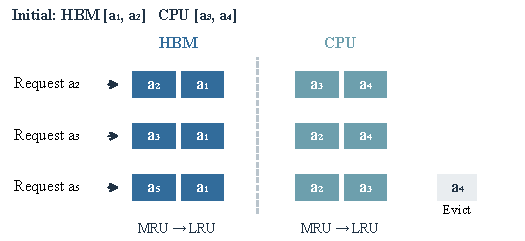
\includegraphics[width=\columnwidth]{method_redesign/residency_cases.pdf}
\par\nointerlineskip
\caption{Three requests from the same initial state. A hit changes recency; a host promotion also demotes the GPU victim; a cold admission can additionally evict the CPU victim. Rows show completed logical states, each ordered MRU to LRU.}
\label{fig:retention}
\end{figure}
Figure~\ref{fig:retention} starts each row from HBM $[a_1,a_2]$ and CPU $[a_3,a_4]$. Requesting $a_2$ changes only HBM recency. Requesting $a_3$ gives HBM $[a_3,a_1]$ and CPU $[a_2,a_4]$. Requesting cold $a_5$ gives HBM $[a_5,a_1]$ and CPU $[a_2,a_3]$; $a_4$ leaves the fast tiers. Promotion preserves the more recent GPU victim in the position vacated on the host.

These completed serial transitions implement exclusive LRU across the combined logical capacity. Batch preparation can promote several experts before their consumers run. The serial stack describes replacement, while the batch path also needs temporary copies and a consumption order. Neither this stack rule nor an initial profile guarantees lower latency on every request stream.

The implementation retains a host mirror with each GPU resident. Demotion can reuse that mirror without D2H. Mirrors add physical host bytes; they do not add logical CPU slots. Logical eviction can release a cache entry before CUDA finishes using its storage. Tensor lifetime must therefore be tracked separately from membership.

\subsection{Ordering Delivery before Expert Consumption}
Prefill identifies the experts selected across its token rows. The runtime submits cold reads for those experts and resolves each read at consumption. Figure~\ref{fig:delivery} shows a prefill schedule in which a resident expert executes while another read progresses. Decode uses demand delivery rather than this prefill read batch. Both paths consume the original gate output and preserve expert aggregation order.

\begin{figure}[H]
\centering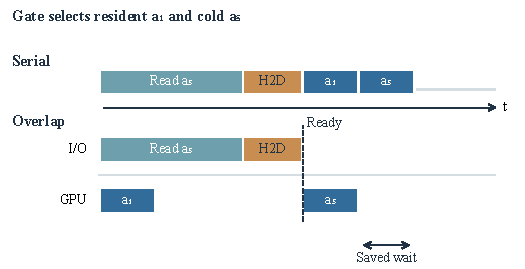
\includegraphics[width=\columnwidth]{method_redesign/delivery_overlap.pdf}
\par\nointerlineskip
\caption{Prefill delivery of resident $a_1$ and cold $a_5$ selected by one gate. Overlap executes ready work during the same read/copy path. The readiness event orders $a_5$'s consumer; the host source remains live through copy completion. Durations are schematic.}
\label{fig:delivery}
\end{figure}
An SSD future must complete before its host weights can be copied. The implementation then waits on the copy stream before yielding CUDA weights to a consumer. Recording the consuming stream prevents allocator reuse while kernels still reference the tensors. These operations enforce read, copy, and use dependencies. The current synchronization covers the copy stream; it is not a per-expert readiness-event scheduler.

The schedule can reduce exposed delivery time without changing which requests miss. Its overlap depends on available resident work and on the submitted read batch. Cache coverage and delivery overlap therefore require separate comparisons.

\subsection{Sharing Execution and Accounting}
Policies share the FP16 loader and router. Accounting distinguishes unique primary residents, host mirrors, and staging storage. Initialization, warmup, prefill, decode, and PPL use separate windows. Logical slot counts describe the replacement experiment; physical allocations describe the host and GPU resources it consumes.

\section{Evaluation}
\label{sec:evaluation}
\subsection{Experimental Setup}
Measured runs use FP16 Mixtral-8x7B-Instruct-v0.1 on one A100 80~GB PCIe. The cold store is on a RAID logical device reporting rotational media; physical drives remain uninventoried. Main runs use four HBM and three host slots per layer, uniform initialization, eight WikiText-2 prompts, 64 input and 64 output tokens, and one run per policy. Perplexity uses 1024 WikiText-2 tokens. The 50/40~GB planner allowances define logical slots; physical allocations also include mirrors and staging buffers.

Yellow-highlighted values and panel titles denote authored illustrative targets, not measurements. The other numerical results are measured A100 outcomes. The experiments address full-system benefit, individual mechanisms, workload change, resource tradeoffs, and numerical equivalence. Streaming loads selected experts on demand without MECC's retention rules. Fixed CPU reserves a static host set; independent caching updates the two fast tiers separately. RF and CPU-compute are local adapters within the shared harness. These controls compare residency and execution decisions under one loader, rather than importing latency numbers from different machines.

\subsection{Single-GPU Performance}
\begin{figure}[H]
\centering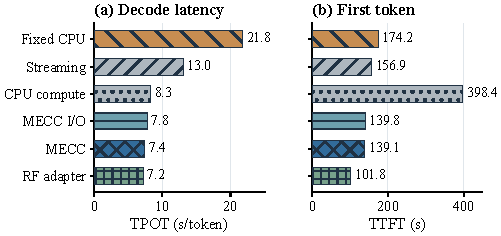
\includegraphics[width=\columnwidth]{measured_figures/main.pdf}
\par\nointerlineskip
\caption{Measured single-A100 runtime: one run per local policy, eight WikiText-2 prompts, 64 output tokens. RF and CPU-compute adapters are local mechanisms.}
\label{fig:performance}
\end{figure}
Figure~\ref{fig:performance} reports MECC at 7.38~s/token, streaming at 13.04, and fixed CPU at 21.75: TPOT ratios of 1.77$\times$ and 2.95$\times$. The RF adapter takes 7.19~s, MECC I/O 7.78, and CPU compute 8.26; the RF adapter is the fastest local variant. MECC's TTFT is 139.1~s, versus 156.9 for streaming and 174.2 for fixed CPU. MECC, streaming, fixed CPU, RF, and MECC I/O report PPL 3.427; CPU compute reports 3.432. The short-window route/logit/token diagnostic agrees between the local streaming and MECC paths.

\subsection{Mechanism Attribution}
\label{sec:mechanisms}
\begin{figure*}[!t]
\centering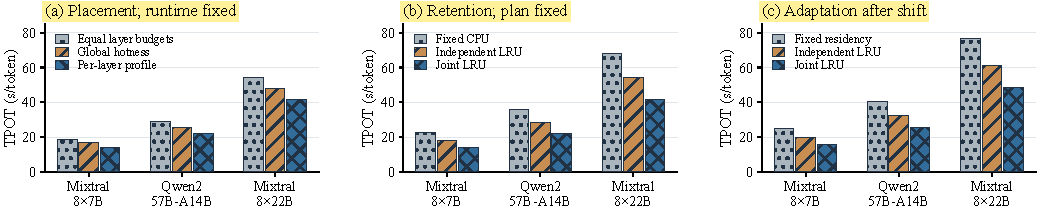
\includegraphics[width=\textwidth]{completion_figures/mechanism_sweeps.pdf}
\par\nointerlineskip
\caption{Component comparisons on three models. (a) Placement with runtime fixed. (b) Retention with initialization fixed. (c) Adaptation after a task switch. The controls isolate initialization, victim retention, and online adaptation, respectively.}
\label{fig:target_mechanisms}
\end{figure*}
The matched local independent-cache control takes 32.94~s/token. Figure~\ref{fig:target_mechanisms} separates three mechanisms in the target component harness. For Mixtral-8x7B, the placement target moves from \pending{18.6 to 14.2 s/token}, joint retention from \pending{18.3 to 14.2}, and post-switch adaptation from \pending{25.1 to 16.0} relative to fixed residency. The three controls hold runtime, initial plan, and switch protocol fixed, respectively. This separates better initial coverage from preservation of later reuse.

\begin{figure}[H]
\centering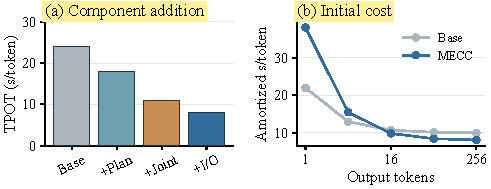
\includegraphics[width=\columnwidth]{completion_figures/ablation_startup.pdf}
\par\nointerlineskip
\caption{Ablation and startup. The right panel reports initialization cost per output token plus decode cost.}
\label{fig:target_ablation}
\end{figure}
Figure~\ref{fig:target_ablation} tests component addition and startup amortization. The authored TPOT sequence is \pending{24, 18, 11, and 8 s/token}. The last I/O step retains a \pending{20-percent target HDD-demand share}, separating delivery scheduling from miss reduction. With the plotted startup/decode costs, the target amortization curves cross at \pending{9 output tokens}. This check exposes the service horizon over which an initial investment pays back.

\begin{figure}[H]
\centering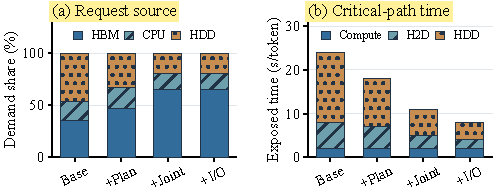
\includegraphics[width=\columnwidth]{completion_figures/traffic_exposure.pdf}
\par\nointerlineskip
\caption{Source demand and exposed time. The last I/O step preserves the demand fractions while shortening the exposed read/copy path.}
\label{fig:target_traffic}
\end{figure}
Figure~\ref{fig:target_traffic} separates cache coverage from scheduling. In the target decomposition, the HDD share falls from \pending{46 to 20 percent} before the I/O step. Overlap then shortens exposed delivery without changing the resident-set result. The stacked latency components sum to the TPOT targets in Figure~\ref{fig:target_ablation}. A source-demand share counts expert requests, while an exposed-time component counts delay on the execution path. Their changes need not be proportional: a host hit still requires H2D, and a cold read may overlap ready GPU work. Keeping both views distinguishes an improvement in cache coverage from an improvement in delivery timing.

\subsection{Model and Deployment Scaling}
\begin{figure}[H]
\centering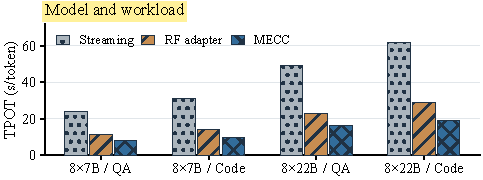
\includegraphics[width=\columnwidth]{completion_figures/cross_model.pdf}
\par\nointerlineskip
\caption{Model and workload comparison. Mixtral-8x7B and 8x22B with QA/code inputs. Each policy uses the same model and workload within a group. The RF policy is a local adapter.}
\label{fig:target_models}
\end{figure}
Figure~\ref{fig:target_models} expands the present one-model workload. The MECC target ranges from \pending{8 to 19 s/token}, versus \pending{24 to 62} for streaming and \pending{11 to 29} for the RF adapter. QA and code exercise different expert-demand patterns; increasing model size also changes the expert pool and transfer size. The comparison therefore pairs every policy within each model/workload point.

\begin{figure}[H]
\centering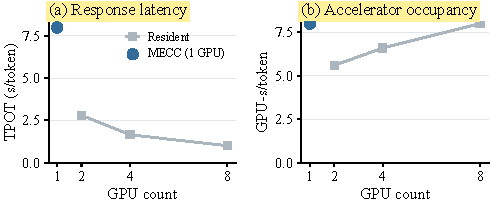
\includegraphics[width=\columnwidth]{completion_figures/gpu_tradeoff.pdf}
\par\nointerlineskip
\caption{One-GPU/resident-reference tradeoff. MECC has only a one-GPU point. Resident points use 2/4/8 GPUs; occupancy is GPU count times TPOT.}
\label{fig:target_gpu}
\end{figure}
Figure~\ref{fig:target_gpu} separates GPU provisioning from response latency. The endpoint target is \pending{one GPU at 8 s/token versus eight GPUs at 1 s/token}; both correspond to \pending{8 GPU-s/token}. The \pending{two-GPU resident target is 5.6 GPU-s/token}, which makes the smallest feasible resident configuration a necessary comparison. Occupancy is reported alongside latency, rather than substituted for energy.

\begin{figure*}[!t]
\centering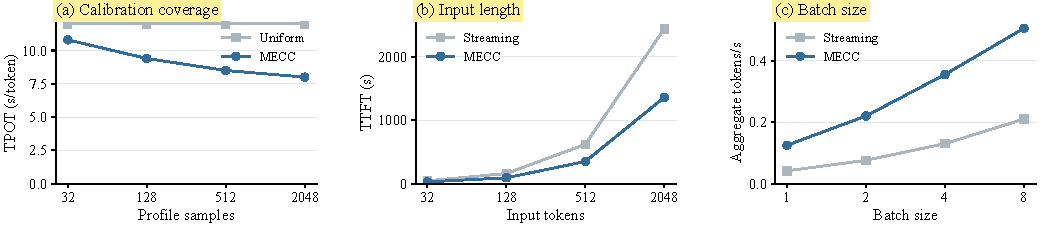
\includegraphics[width=\textwidth]{completion_figures/workload_sensitivity.pdf}
\par\nointerlineskip
\caption{Profile, input-length, and batch sensitivity. Profile size changes initialization quality, input length changes first-token work, and batch size changes aggregate throughput. The panels vary one workload parameter at a time.}
\label{fig:target_sensitivity}
\end{figure*}
\subsection{Capacity and Workload Sensitivity}

The measured 30/60~GB settings give MECC TPOTs of 14.46 and 0.76~s/token, with 32.2\% and zero HDD demand. Four HBM plus four host slots at 60~GB cover all eight experts per layer; zero cold demand is a capacity transition. RF takes 13.06 and 0.74~s/token. These points use a shorter protocol than the main run.

\begin{figure}[H]
\centering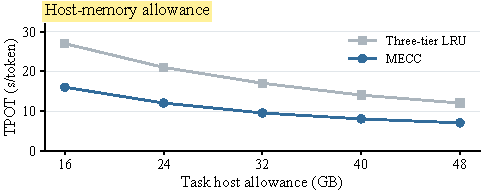
\includegraphics[width=\columnwidth]{completion_figures/quota_targets.pdf}
\par\nointerlineskip
\caption{Host-memory allowance sweep. Five host allowances compare MECC and three-tier LRU within one comparison protocol.}
\label{fig:target_quota}
\end{figure}
Figure~\ref{fig:target_quota} resolves intermediate capacity points. Its authored MECC target changes from \pending{16 to 7 s/token} over \pending{16--48 GB}, compared with \pending{27 to 12} for three-tier LRU. The purpose is to separate pressure within the cold-tier regime from the full-coverage threshold. Additional host capacity can first preserve more reused victims, then eliminate cold demand once the complete expert set fits. The latter transition changes the dominant delivery path from HDD plus H2D to H2D alone. It explains why capacity and replacement policy must be examined together instead of extrapolating one speedup across all allowances.






\begin{figure}[H]
\centering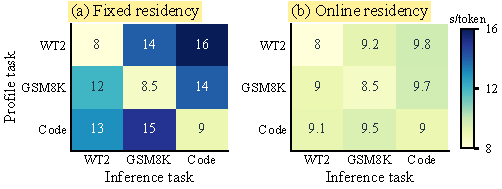
\includegraphics[width=\columnwidth]{completion_figures/profile_mismatch.pdf}
\par\nointerlineskip
\caption{Profile transfer across tasks. Rows select the calibration task and columns the inference task. Cells are TPOT in s/token; the two panels share a color scale.}
\label{fig:target_mismatch}
\end{figure}
Figure~\ref{fig:target_sensitivity} examines scale within a workload. Figure~\ref{fig:target_mismatch} examines transfer between WikiText-2, GSM8K, and code inputs. Its target pattern distinguishes a useful initial prior from a permanently fixed placement: online membership updates reduce the off-diagonal penalty while retaining the matched-profile behavior.

\balance
\section{Related Work}
\textbf{Layer planning and online residency.} MoE-CORE combines nonuniform device capacity, domain-informed initialization, routing-history-aware replacement, and cross-layer prefetching~\cite{core}. Its main path executes the router-selected experts; substitution is optional. MECC also separates initialization from online membership. Its focus is the connection between per-layer allocation and joint HBM/CPU retention when a selected expert can miss both tiers. Their overlap directs attention to the initial state, victim rule, and delivery path used by each comparison.

\textbf{Storage-backed expert delivery.} SSD-LLaMA manages bounded RAM and VRAM caches, retains GPU victims on the host when possible, and pipelines expert reads and transfers~\cite{ssdllama}. It also studies lossless transport compression and CPU/GPU execution partitioning. Edge FlashMoE studies device-cache replacement with on-demand storage access~\cite{flashmoe}. MECC keeps FP16 representation and GPU expert execution fixed in its retention controls. Fixing representation and execution placement isolates the residency decision within the shared delivery stack.

\textbf{Offloading, prediction, and execution.} Early expert offloading and SwapMoE expose placement and paging choices~\cite{offloading,swapmoe}. Fiddler and DAOP choose CPU/GPU work; MoE-Lightning pipelines heterogeneous execution; MoE-Infinity uses activation traces~\cite{fiddler,daop,lightning,moeinfinity}. ProMoE, Pre-gated MoE, Fate, and ExpertFlow use proactive caching, lookahead, or token scheduling~\cite{promoe,pregated,fate,expertflow}. HOBBIT and Specter vary loading precision; MoEpic uses segments; SliceMoE uses precision slices; Mira combines staging and quantization~\cite{hobbit,specter,moepic,slicemoe,mira}. ZipMoE uses compression and affinity scheduling~\cite{zipmoe}. These mechanisms change demand prediction, bytes per request, or where computation runs. A comparison of whole-expert retention keeps those choices fixed.

Klotski and Bevy expose work across batches or requests~\cite{klotski,bevy}. OD-MoE distributes on-demand loading across edge nodes; HeteGen studies heterogeneous dense inference~\cite{odmoe,hetegen}. Their scheduling scopes differ from delivery within the current MoE gate. Ready work from another request can hide a wait even when the ongoing request has no resident expert to execute. This distinction separates throughput from the response time of one request.

\section{Conclusion}
MECC connects profile-guided placement, online cross-tier retention, and expert delivery for HDD-backed single-GPU MoE inference. Per-layer compilation improves the initial use of bounded capacity. Joint retention preserves reuse after GPU eviction, and readiness-aware delivery overlaps available work with weight movement. The A100 implementation characterizes these decisions through runtime latency, source-tier demand, capacity sensitivity, and numerical comparisons under a shared FP16 execution harness.

\clearpage
\nobalance
\IEEEtriggeratref{24}
\bibliographystyle{IEEEtran}
\bibliography{references}
\end{document}
